%%%%%%%%%%%%%%%%%%%%%%%%%%%%%%%%%%%%%%%%%%%%%%%%%%%%%%%%%%%%%%
%%%                                                        %%%
%%%        IMPORTANT - DO NOT ADD EXERCISES HERE           %%%
%%%                                                        %%%
%%%    ALL EXERCISES MUST FIRST GO TO SOLUTION MANUAL,     %%%
%%%       THEN STRIPPED OFF SOLUTIONS AND GO HERE          %%%
%%%                                                        %%%
%%%%%%%%%%%%%%%%%%%%%%%%%%%%%%%%%%%%%%%%%%%%%%%%%%%%%%%%%%%%%%

%%%%%%%%%%%%%%%%%%%%%%%%%%%%%%%%%%%%%%%%%%%%%%%%%%%%%%%%%%%%%%%%%%%%%%%%%%%%%%%%%%%%%%%%%%
\setcounter{section}{2}
\section{Manual Mode}

All exercises in this textbook are available for download in NCLab's
public database (in fact they might be in newer version there). 
To load them into your NCLab account, launch the File Manager, go
to the File menu and click on Search. Enter the exercise number of 
name into the search box that appears. You are likely to see copies
-- originals are provided by Karel Team.  

\subsection{Get going!}

{\em In every game, your goal is to guide Karel to his home square. Sometimes you will need to fulfill additional tasks, but not now. After pressing Start, five buttons appear and your time counter is on. Good luck!}\\[-7mm]
\begin{figure}[!ht]
\begin{center}
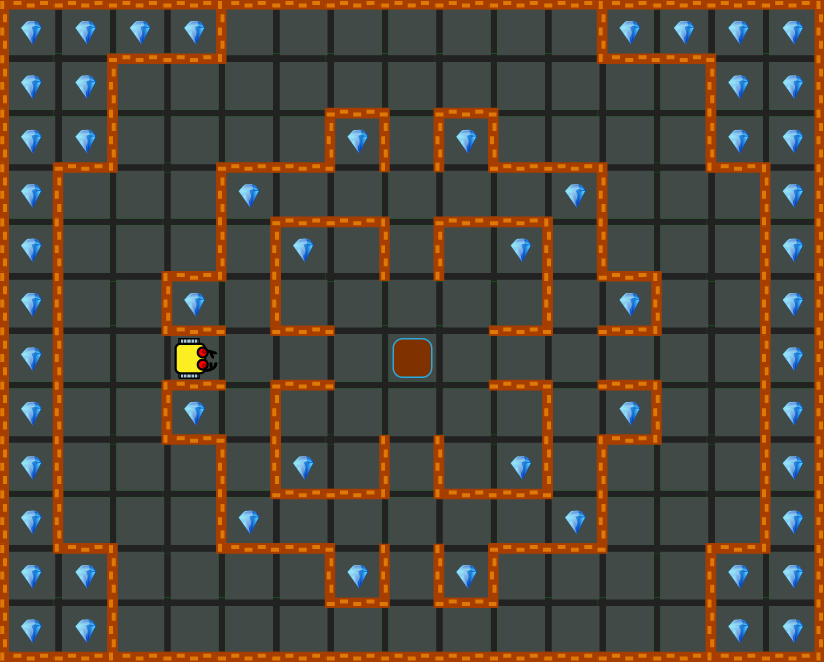
\includegraphics[height=0.4\textwidth]{img/a01.png}
\end{center}
\vspace{-4mm}
\caption{Help the robot get home before his batteries run out!}
\label{fig:a01}
\end{figure}

\noindent
Pressing Start will start the game, and at this time also the buttons 
Go, Left, Right, Put and Get appear, as shown in Fig. \ref{fig:buttons2222}.\\[-7mm]

\begin{figure}[!ht]
\begin{center}
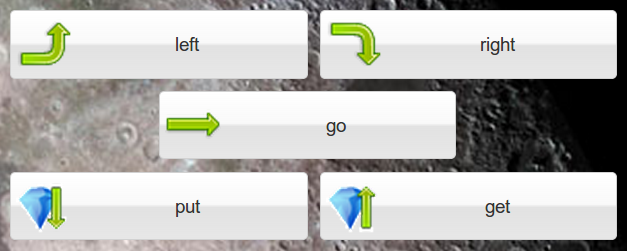
\includegraphics[width=5cm]{img/buttons-all.png}
\vspace{-0mm}
\caption{Karel can be guided manually, using five buttons located in the left panel.}
\vspace{-1.2cm}
\label{fig:buttons2222}
\end{center}
\end{figure}


\newpage
\subsection{1st olympic games}

{\em Karel is training for Robolympic Games! Your task is to run as fast as possible. Karel's personal record is three seconds.}

\begin{figure}[!ht]
\begin{center}
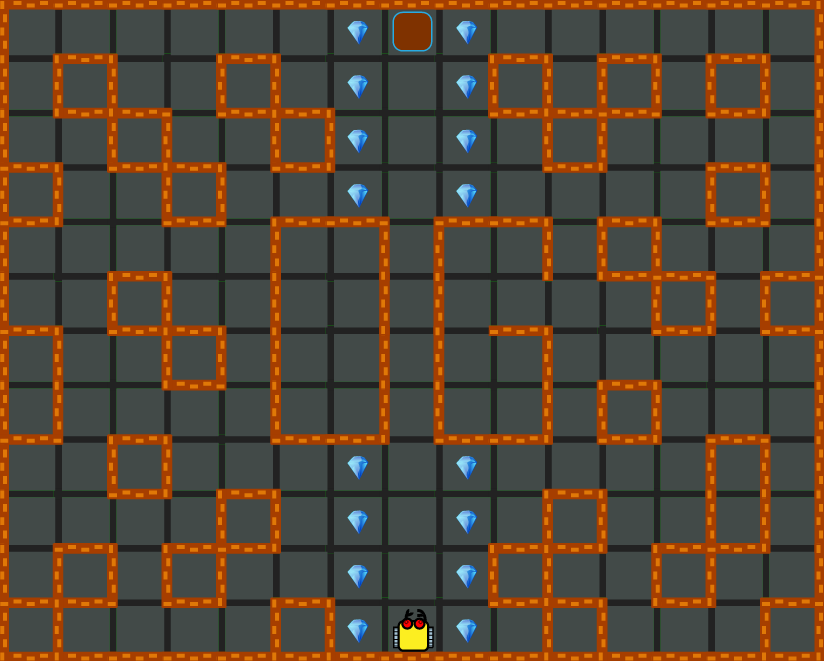
\includegraphics[height=0.4\textwidth]{img/a02.png}
\end{center}
\vspace{-4mm}
\caption{Karel is training for Robolympic Games.}
\label{fig:a02}
\vspace{-4mm}
\end{figure}
\noindent

\subsection{First gem}

{\em Today Karel is about to get his first gem. Do not forget to pick it up!}

\begin{figure}[!ht]
\begin{center}
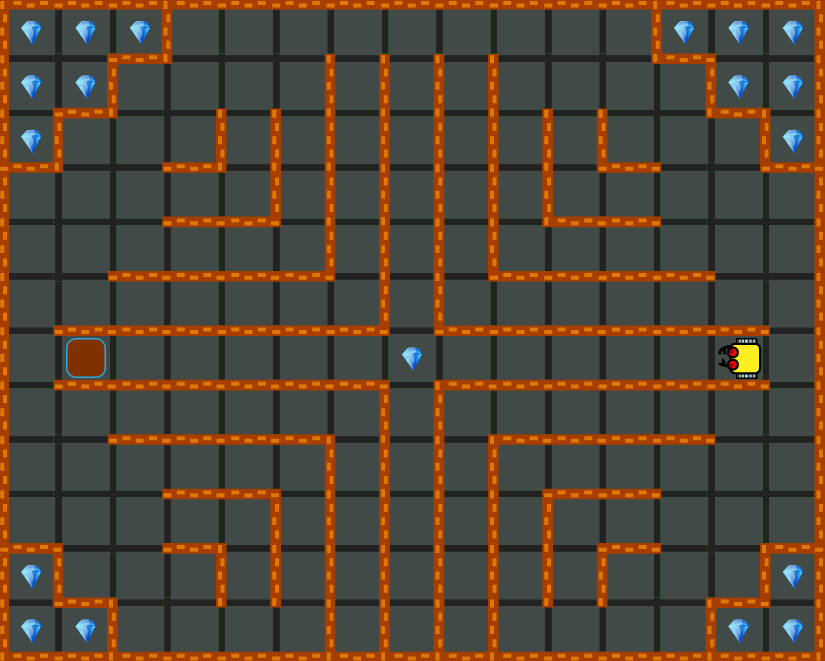
\includegraphics[height=0.4\textwidth]{img/a03.png}
\end{center}
\vspace{-4mm}
\caption{Karel is about to collect his first gem!}
\label{fig:a03}
\vspace{-1cm}
\end{figure}
\noindent

\subsection{2nd olympic games}

{\em It is Robolympic season again! Run as fast as you can, and collect all three gems on the way. Karel's personal record is 10 seconds.}


\begin{figure}[!ht]
\begin{center}
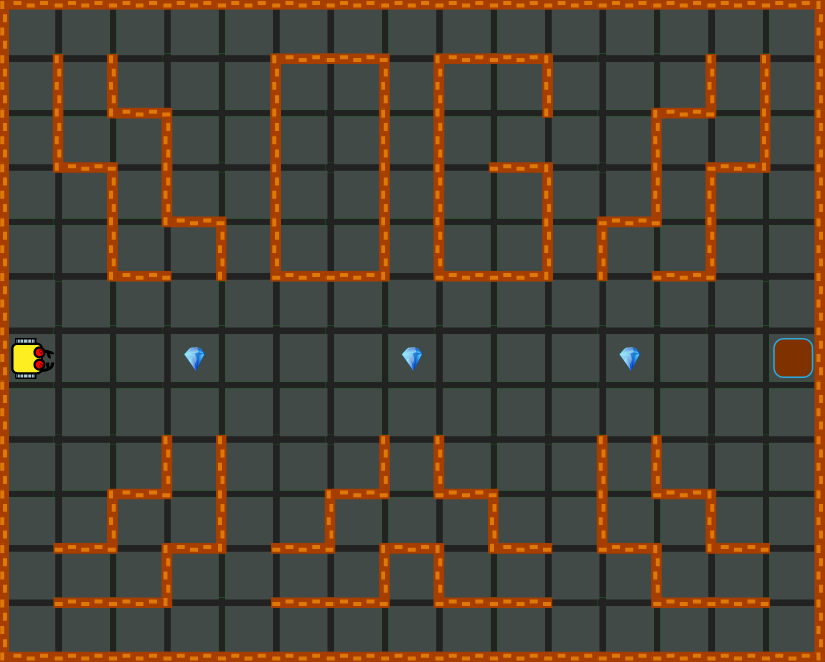
\includegraphics[height=0.4\textwidth]{img/a04.png}
\end{center}
\vspace{-4mm}
\caption{Karel's second Robolympic Games.}
\label{fig:a04}
\vspace{-1cm}
\end{figure}
\noindent


\subsection{Taking turns}

{\em Your task is to collect just one gem, but your battery is good for only 10 steps. Good luck!}

\begin{figure}[!ht]
\begin{center}
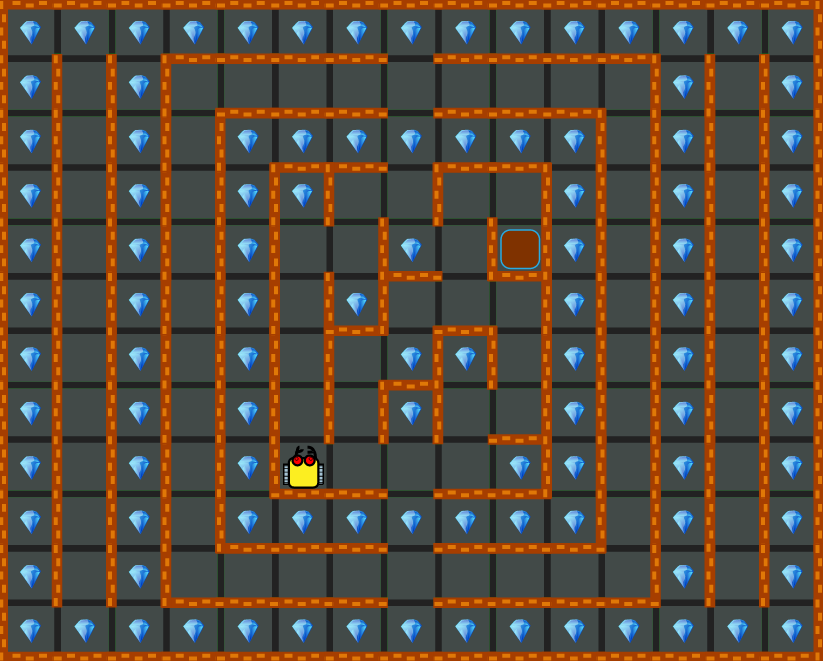
\includegraphics[height=0.4\textwidth]{img/a05.png}
\end{center}
\vspace{-4mm}
\caption{Karel is about to practice some turns!}
\label{fig:a05}
\vspace{-1cm}
\end{figure}
\noindent


\subsection{3rd olympic games}

{\em Karel is training for his third Robolympic Games. Run around the block as fast as you can, and collect at least one gem! Karel's personal record is 16 seconds.}

\begin{figure}[!ht]
\begin{center}
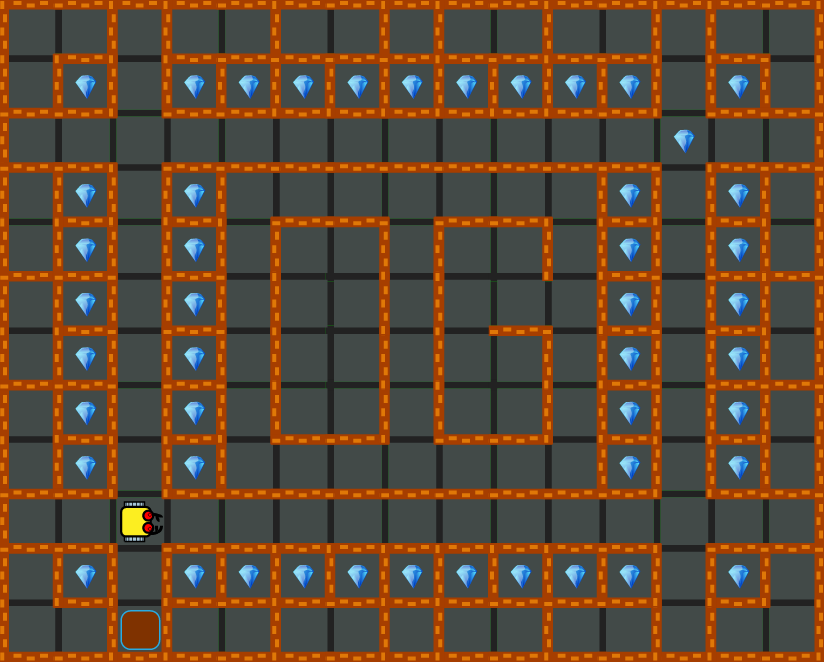
\includegraphics[height=0.4\textwidth]{img/a06.png}
\end{center}
\vspace{-4mm}
\caption{Karel's third Robolympic Games.}
\label{fig:a06}
\vspace{-1cm}
\end{figure}
\noindent


\subsection{Head spin}

{\em Now this will require some turning! You need to collect twelve gems. Do not make a false step!}

\begin{figure}[!ht]
\begin{center}
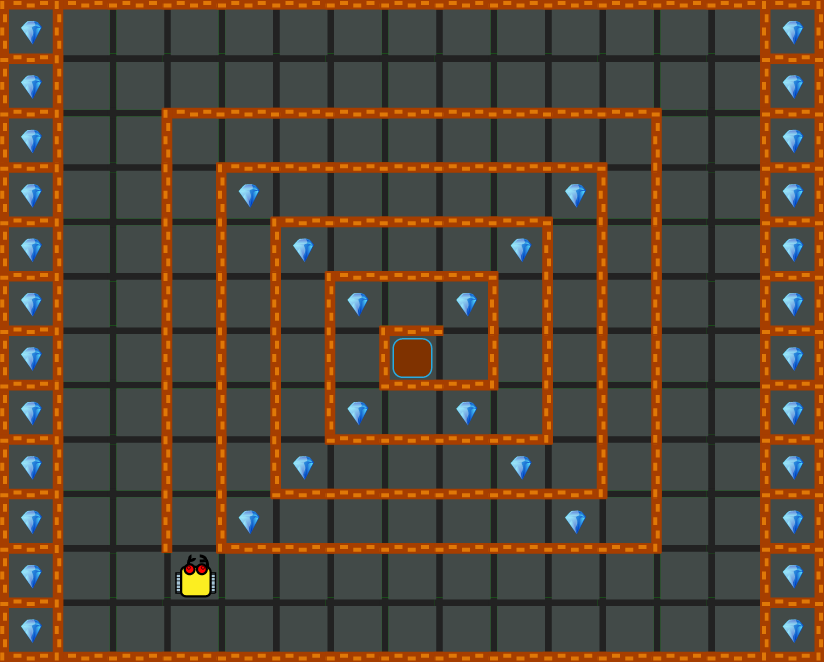
\includegraphics[height=0.4\textwidth]{img/a07.png}
\end{center}
\vspace{-4mm}
\caption{Karel is getting a head spin.}
\label{fig:a07}
\vspace{-1cm}
\end{figure}
\noindent

\subsection{4th olympic games}

{\em Last season of Karel's Robolympics Games is here! The robot needs to run home as fast as possible and bring one gem. Be careful not to crash, this is a tricky level! Karel's personal record is 25 seconds.}\\[-7mm]

\begin{figure}[!ht]
\begin{center}
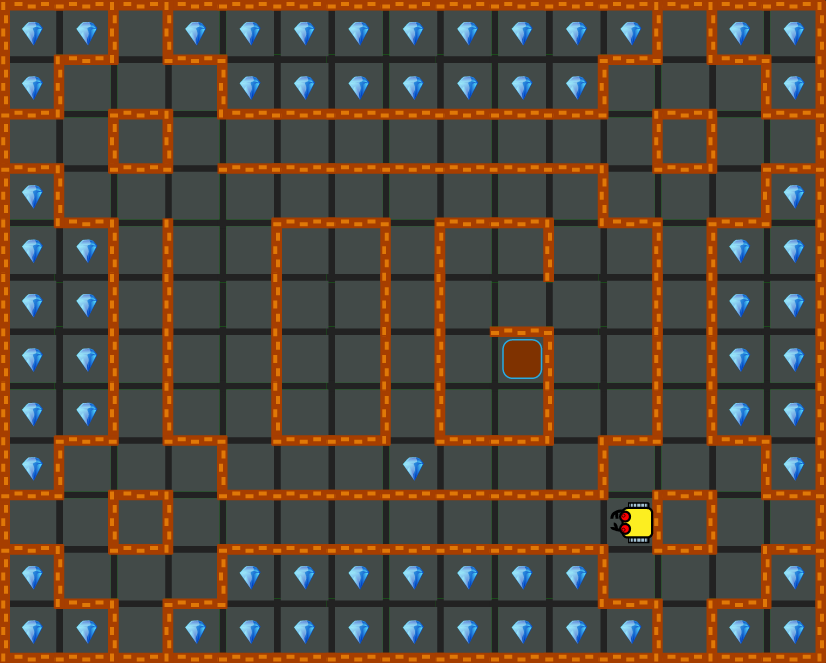
\includegraphics[height=0.4\textwidth]{img/a08.png}
\end{center}
\vspace{-4mm}
\caption{Karel's fourth Robolympic Games.}
\label{fig:a08}
\vspace{-4mm}
\end{figure}
\noindent

\subsection{Mad maze man}

{\em This is the most challenging level yet. Karel needs to collect five gems before he gets to his home square,}\\[-7mm]

\begin{figure}[!ht]
\begin{center}
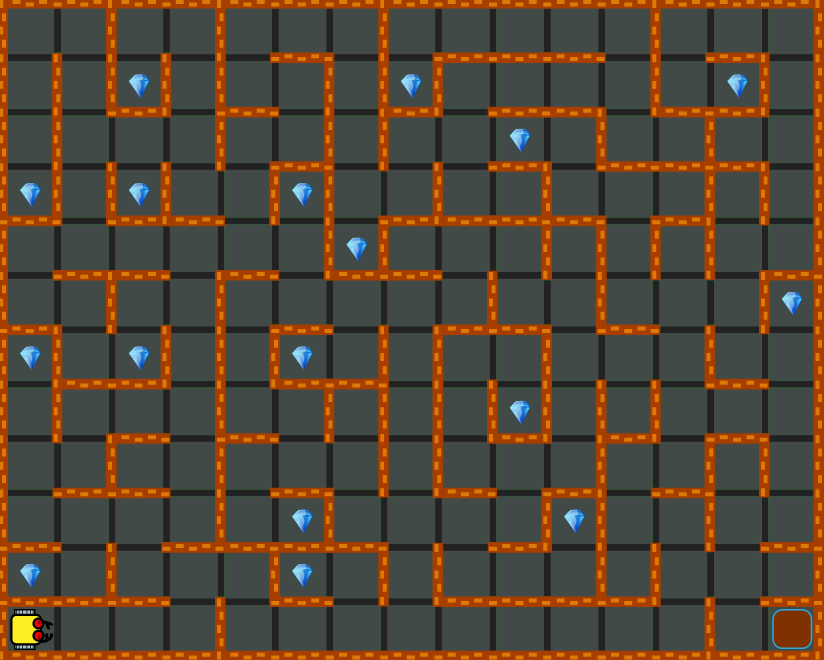
\includegraphics[height=0.4\textwidth]{img/a09.png}
\end{center}
\vspace{-4mm}
\caption{Karel needs to collect five gems in this mad maze.}
\label{fig:a09}
\vspace{-10mm}
\end{figure}
\noindent
\newpage

\subsection{Labyrinth quest}

{\em This is a true labyrinth. As usual, your task is to lead Karel home. There is no rush, you have enough time, but every step counts!}

\begin{figure}[!ht]
\begin{center}
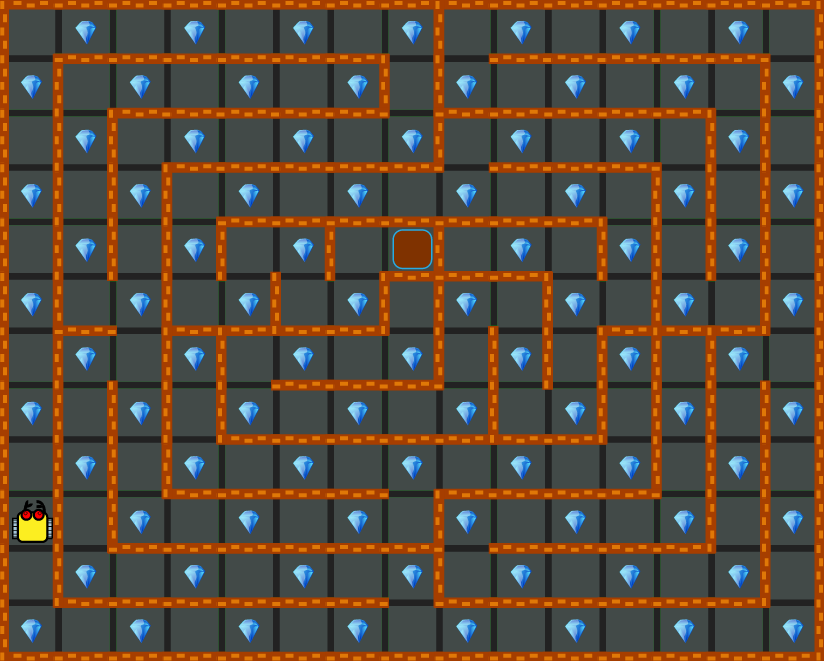
\includegraphics[height=0.4\textwidth]{img/a10.png}
\end{center}
\vspace{-4mm}
\caption{Karel needs to find his way home in a labyrinth.}
\label{fig:a10}
\vspace{-4mm}
\end{figure}
\noindent


\subsection{Diamond mine}

{\em Karel discovered an abandoned diamond mine. Collect all nine gems and get back home in time!}

\begin{figure}[!ht]
\begin{center}
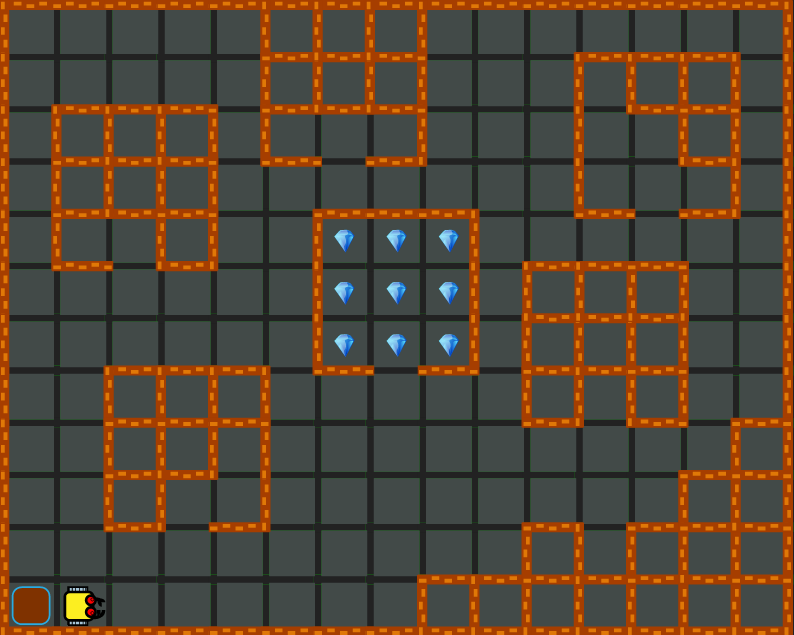
\includegraphics[height=0.4\textwidth]{img/a11.png}
\end{center}
\vspace{-4mm}
\caption{Karel found an abandoned diamond mine.}
\label{fig:a11}
\vspace{-10mm}
\end{figure}
\newpage
\noindent

\subsection{Diamond desk}

{\em Karel has nine gems in his bag. Put all of them on the table and get Karel to his home square!}

\begin{figure}[!ht]
\begin{center}
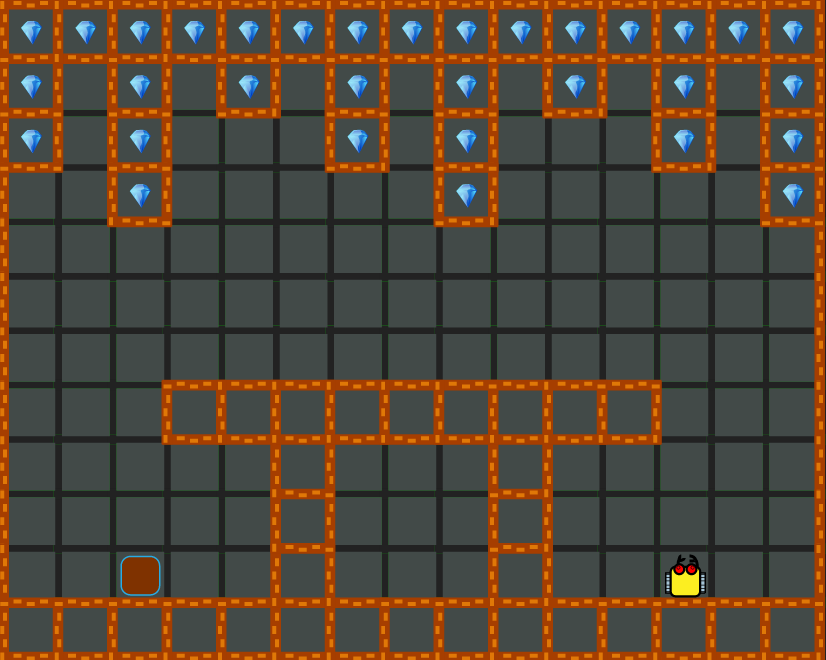
\includegraphics[height=0.4\textwidth]{img/a13.png}
\end{center}
\vspace{-4mm}
\caption{Karel needs to put five gems on the table.}
\label{fig:a13}
\vspace{-4mm}
\end{figure}
\noindent
\newpage

%%%%%%%%%%%%%%%%%%%%%%%%%%%%%%%%%%%%%%%%%%%%%%%%%%%%%%%%%%%%%%%%%%%%%%%%%%%%%%%%%%%%%%%%%%

\section{Programming Mode 1 - Simple commands}

\subsection{Force of Darkness}

{\em The Force of Darkness already took most of Karel's world. You are his only ally and last hope. Write a program that gets Karel home! Remember: The keywords displayed on the five buttons in the manual mode are Karel's basic commands. Always type one command per line.}\\[-8mm]

\begin{figure}[!ht]
\begin{center}
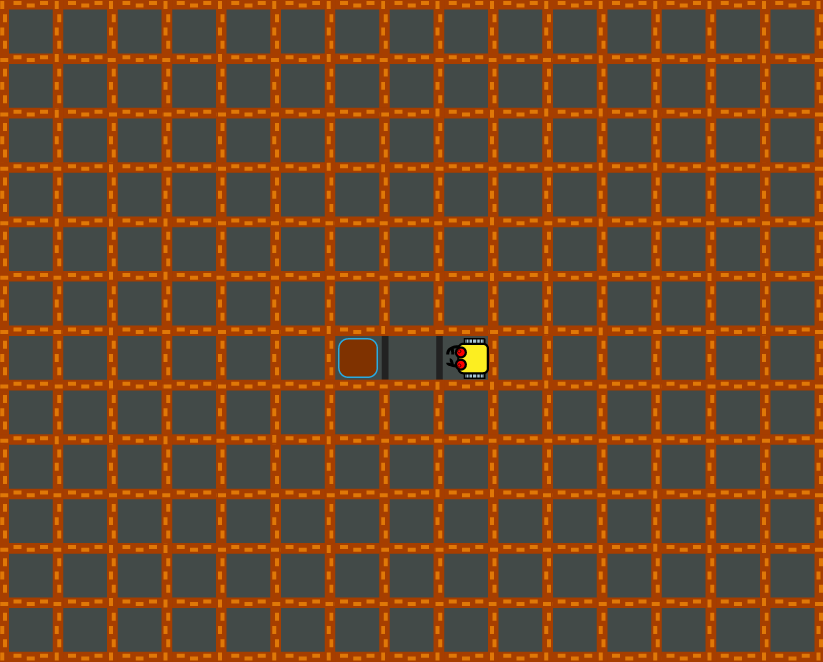
\includegraphics[height=0.4\textwidth]{img/b01.png}
\end{center}
\vspace{-4mm}
\caption{Rescuing Karel from the Force of Darkness.}
\label{fig:b01}
\vspace{-9mm}
\end{figure}
\noindent

\subsection{Pyrotechnist}

{\em Karel is a pyrotechnist. The only way to avoid a catastrophic explosion is to collect three detonators (gems) and enter his home square quickly. Many lives depend on you, good luck!}\\[-8mm]

\begin{figure}[!ht]
\begin{center}
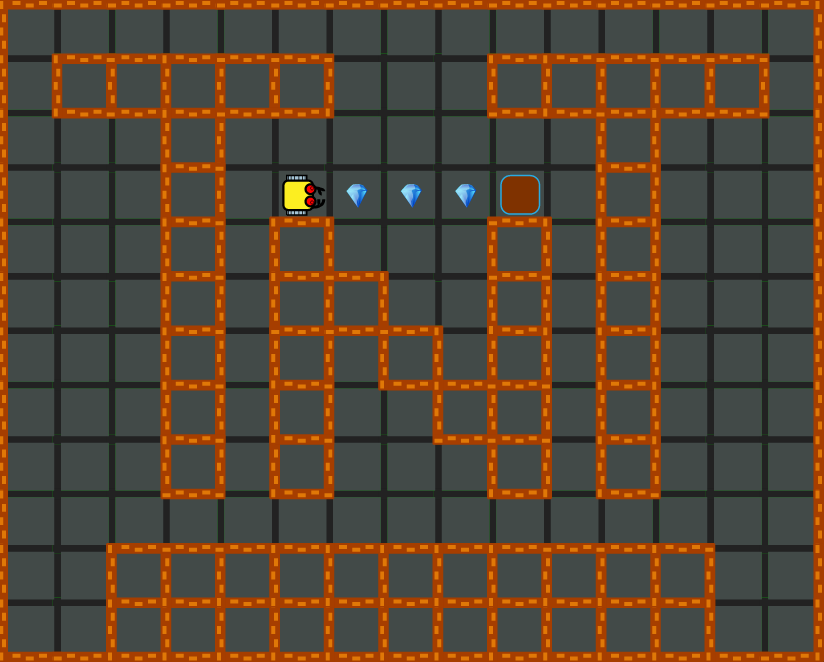
\includegraphics[height=0.4\textwidth]{img/b02.png}
\end{center}
\vspace{-4mm}
\caption{Avoiding catastrophic explosion.}
\label{fig:b02}
\vspace{-1.2cm}
\end{figure}
\newpage


\subsection{Ballet}

{\em Karel is practicing ballet moves by collecting a gem that is positioned diagonally between him and his home square.}

\begin{figure}[!ht]
\begin{center}
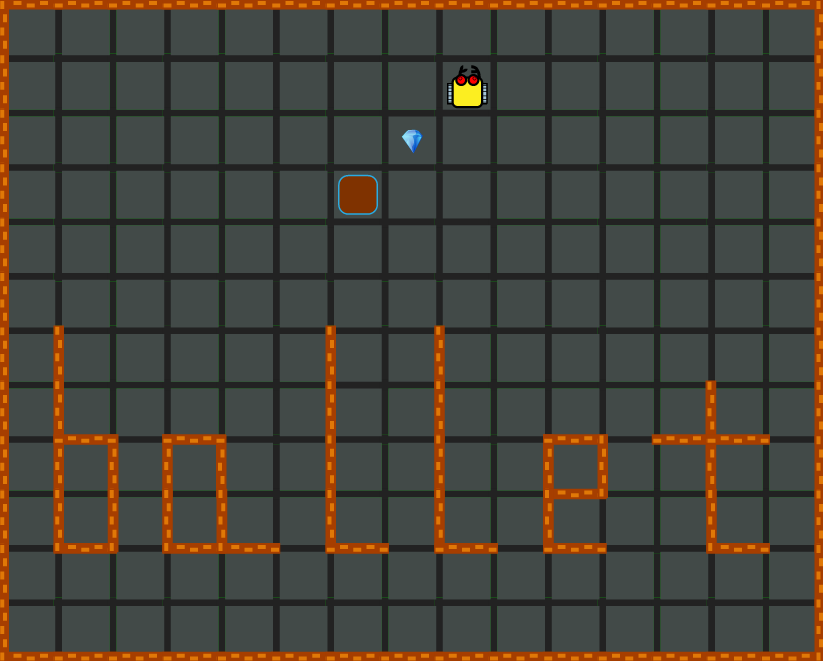
\includegraphics[height=0.4\textwidth]{img/b03.png}
\end{center}
\vspace{-4mm}
\caption{Practicing ballet moves.}
\label{fig:b03}
\vspace{-1cm}
\end{figure}

\subsection{Kung-fu}
{\em Karel is training advanced kung-fu techniques. He needs to neutralize four enemy fighters (collect four gems) before entering his home square.}

\begin{figure}[!ht]
\begin{center}
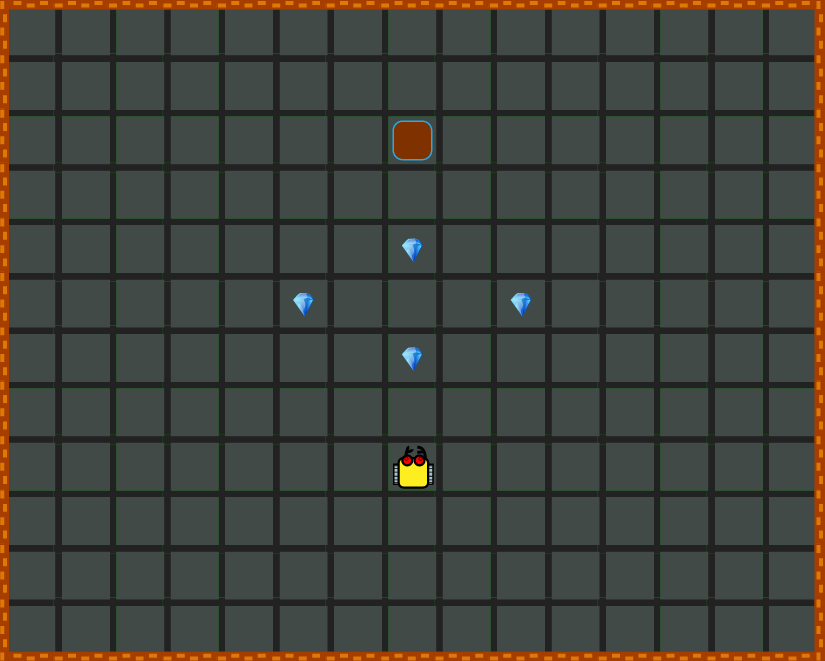
\includegraphics[height=0.4\textwidth]{img/a19.png}
\end{center}
\vspace{-4mm}
\caption{Karel is training kung-fu.}
\label{fig:b06}
\vspace{-10mm}
\end{figure}

%%%%%%%%%%%%%%%%%%%%%%%%%%%%%%%%%%%%%%%%%%%%%%%%%%%%%%%%%%%%%%%%%%%%%%%%%%%%%%%%%%%%%%%%%%

\setcounter{section}{4}
\section{Programming Mode 1 - Counting Loop}

\subsection{Efficiency}

{\em Karel is in a random maze. His home square is ten steps away and there are no obstacles on the way. Use the {\tt repeat} command to get Karel home with only {\bf two lines of code}!}\\[-7mm]

\begin{figure}[!ht]
\begin{center}
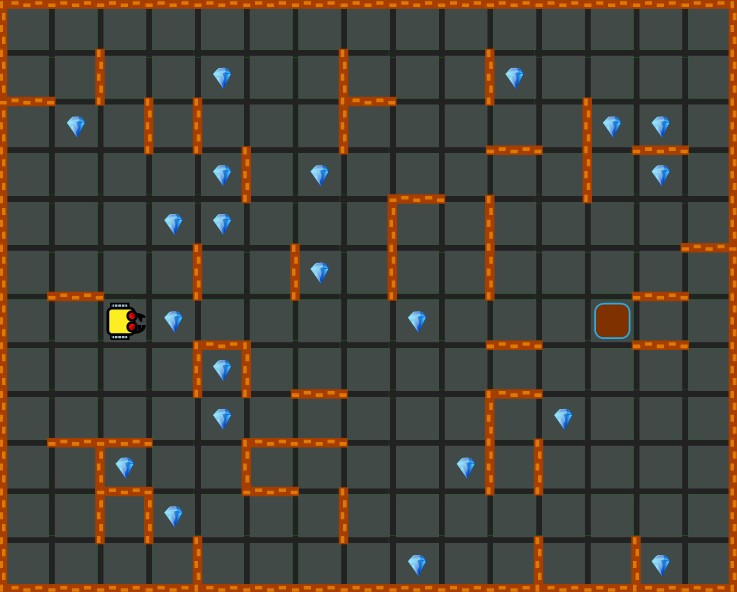
\includegraphics[height=0.4\textwidth]{img/c01.png}
\end{center}
\vspace{-4mm}
\caption{Help Karel get home efficiently, using only two lines of code!}
\label{fig:c01}
\vspace{-1cm}
\end{figure}


\subsection{Diamond streak}

{\em Collect all 11 gems before entering the home square! Your program should not be longer than {\bf six lines}.}\\[-7mm]

\begin{figure}[!ht]
\begin{center}
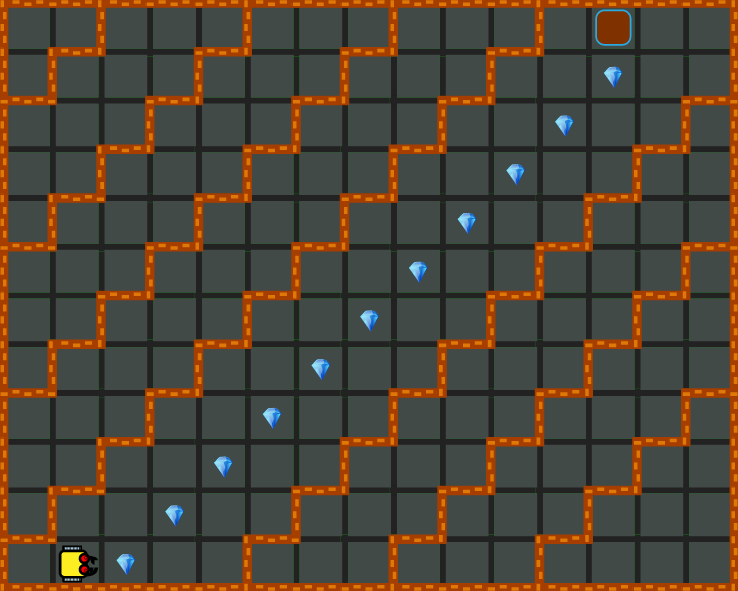
\includegraphics[height=0.4\textwidth]{img/c02.png}
\end{center}
\vspace{-4mm}
\caption{There is a diamond streak between Karel and his home.}
\label{fig:c02}
\vspace{-10mm}
\end{figure}
\noindent

\newpage

\subsection{Visit to Idaho}

{\em Karel is helping his friends in Idaho to harvest potatoes. There are six trenches with 10 potatoes (gems) each. Write a program to collect all potatoes and enter the home square. Your program should have at most {\bf 15 lines}.}\\[-7mm]

\begin{figure}[!ht]
\begin{center}
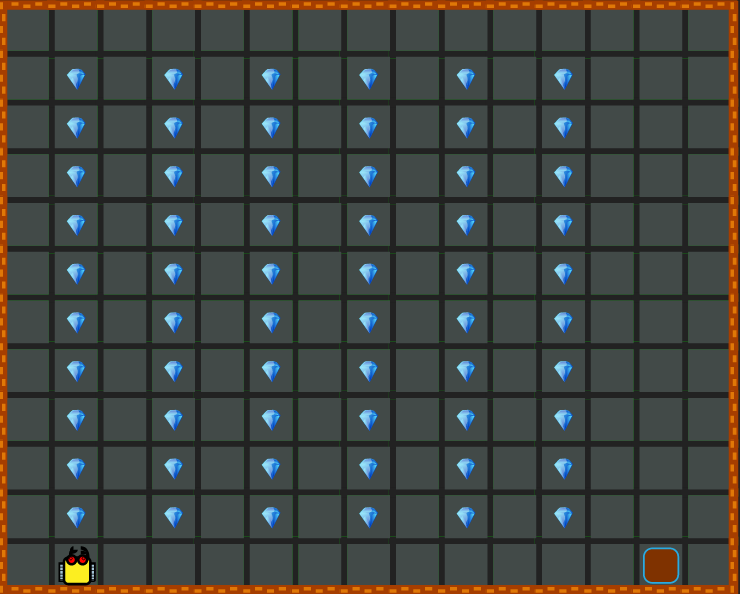
\includegraphics[height=0.4\textwidth]{img/c03.png}
\end{center}
\vspace{-4mm}
\caption{Karel is harvesting potatoes in Idaho.}
\label{fig:c03}
\vspace{-10mm}
\end{figure}
\noindent

\subsection{Fortress}

{\em This is your final task in Programming Mode 1. Let's finish in style! Karel needs to collect all 138 gems and enter his home square in the heart of the fortress. Your program should not have more than {\bf 20 lines}. You may want to change the robot's speed to Fast in Settings.}\\[-9mm]

\begin{figure}[!ht]
\begin{center}
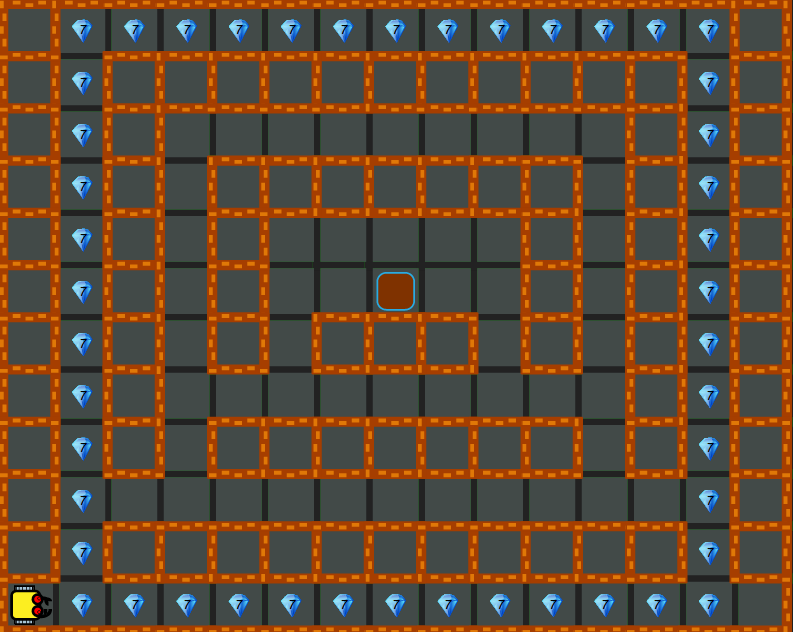
\includegraphics[height=0.4\textwidth]{img/a28.png}
\end{center}
\vspace{-5mm}
\caption{Final task in Programming Mode 1.}
\label{fig:a28}
\vspace{-10mm}
\end{figure}

%%%%%%%%%%%%%%%%%%%%%%%%%%%%%%%%%%%%%%%%%%%%%%%%%%%%%%%%%%%%%%%%%%%%%%%%%%%%%%%%%%%%%%%%%%

\setcounter{section}{6}
\section{Programming Mode 2 - Conditions}

\subsection{Holey pocket!}

{\em Because of a hole in his pocket, Karel just lost some gems. They lie at random positions between him and his home which is 10 steps away. Go back and collect all of them quickly! Your program should have at most {\bf four lines}.}\\[-9mm]

\begin{figure}[!ht]
\begin{center}
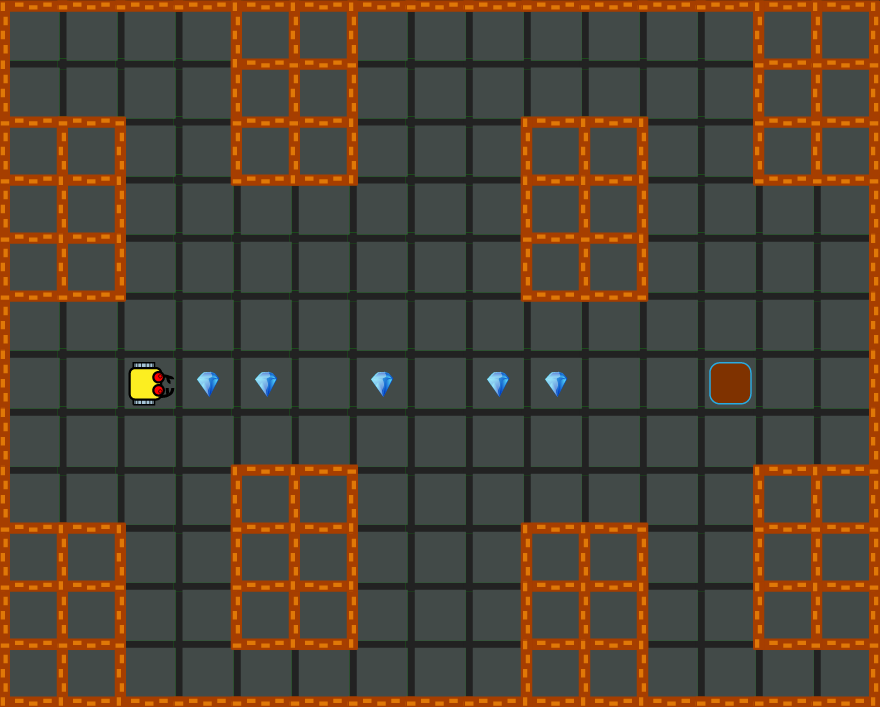
\includegraphics[height=0.4\textwidth]{img/d01.png}
\end{center}
\vspace{-5mm}
\caption{Karel needs to recover gems that he lost.}
\label{fig:d01}
\vspace{-1.3cm}
\end{figure}


\subsection{Librarian}

{\em The library aisle has 10 slots for books (represented by gems). Several of them are empty, and the number and position of the empty ones are random. Karel's task is to fill all empty slots and enter his home square. Your program should have at most {\bf 10 lines}.}\\[-9mm]


\begin{figure}[!ht]
\begin{center}
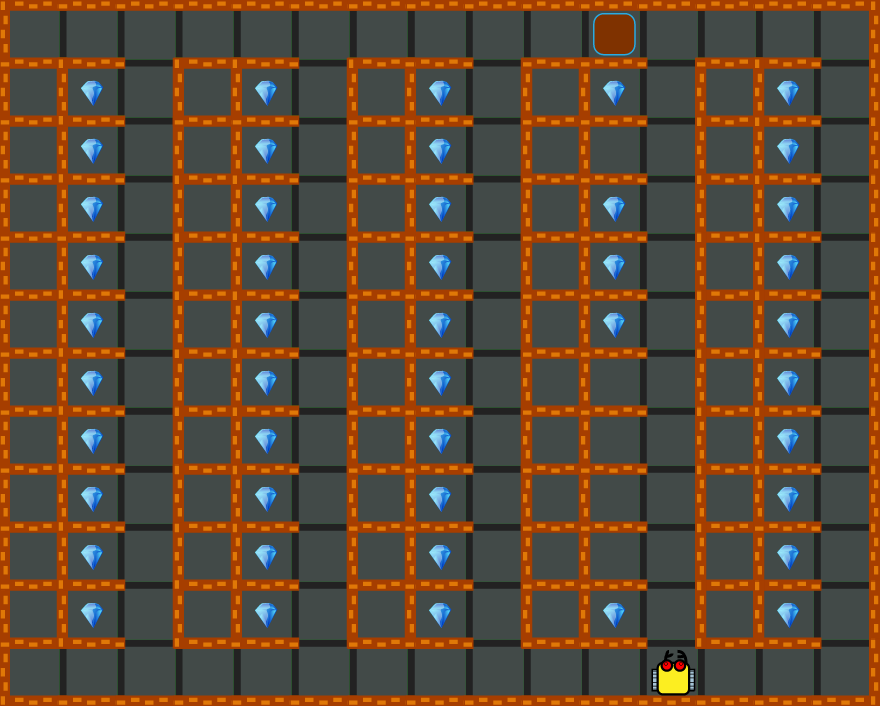
\includegraphics[height=0.4\textwidth]{img/d02.png}
\end{center}
\vspace{-4mm}
\caption{Karel works at a library.}
\label{fig:d02}
\vspace{-12mm}
\end{figure}
\newpage


\subsection{Archeologist}

{\em Karel works at an archeological site. His home is 11 steps straight ahead but he cannot just walk over there because of three impassable excavations which are in his way. These obstacles are at random positions. There are never excavations in adjacent squares. Write a program for Karel to reach his home square collecting all gems that he finds on the way!}\\[-7mm]

\begin{figure}[!ht]
\begin{center}
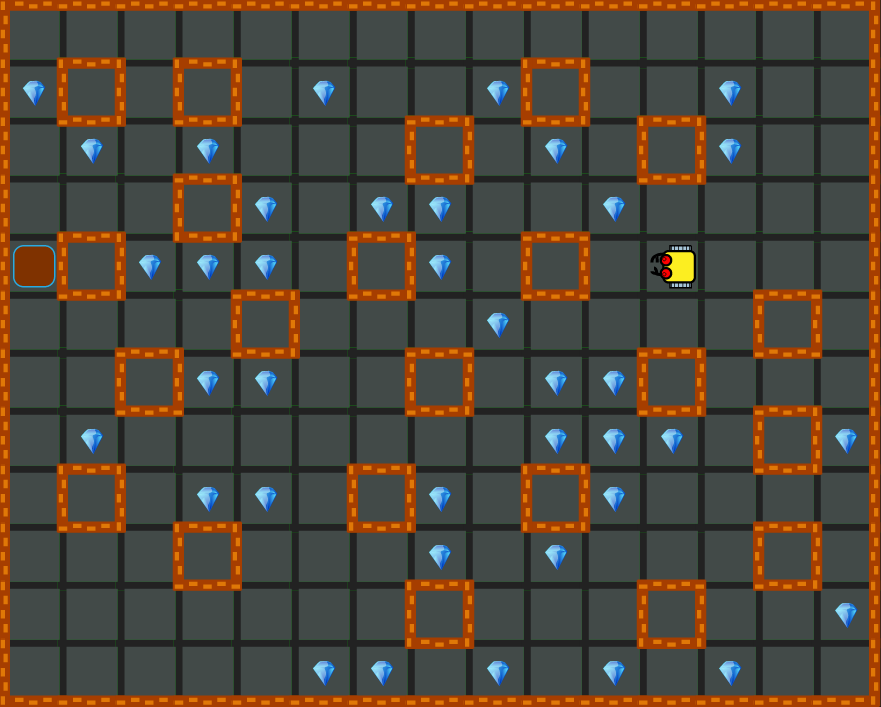
\includegraphics[height=0.4\textwidth]{img/d03.png}
\end{center}
\vspace{-4mm}
\caption{Karel is an archeologist.}
\label{fig:d03}
\vspace{-10mm}
\end{figure}


\subsection{Treasure of the Pharaohs}

{\em Karel is hunting for the legendary Treasure of the Pharaoh's. He is almost there - one last deadly trap awaits him! He stands in complete darkness, at the cross-section of four tunnels. He is facing a random direction - either North, West, South or East. He knows that the West tunnel leads to the treasure while the remaining three contain a metal-eating bacteria that would destroy him. Using the map of the pyramid that you can see, write a program for Karel to collect all gems and enter his home square! Can you do it using just {\bf 11 lines of code} and not use the {\tt while} command?}
\newpage


\vspace{-5mm}
\begin{figure}[!ht]
\begin{center}
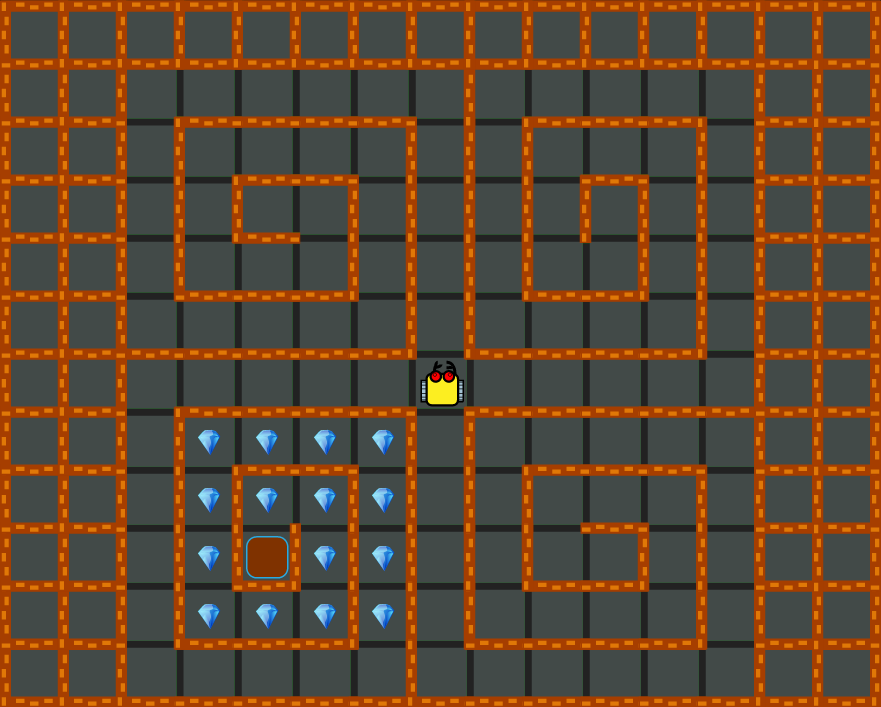
\includegraphics[height=0.4\textwidth]{img/d04.png}
\end{center}
\vspace{-4mm}
\caption{Treasure of the Pharaohs.}
\label{fig:d04}
\vspace{-10mm}
\end{figure}

%%%%%%%%%%%%%%%%%%%%%%%%%%%%%%%%%%%%%%%%%%%%%%%%%%%%%%%%%%%%%%%%%%%%%%%%%%%%%%%%%%%%%%%%%%

\section{Programming Mode 2 - Conditional Loop}

\subsection{Hide and seek}

{\em Karel is playing hide-and-seek with his friends. They left on the ground a chain of gems that will help the robot find them. They gave Karel the following instructions: He should walk straight ahead, and whenever he finds a gem, he should turn left and walk straight ahead again. Write a program for Karel to do this, and do not forget to collect all gems on the way! Your program should have at most {\bf 5 lines}.}\\[-7mm]

\begin{figure}[!ht]
\begin{center}
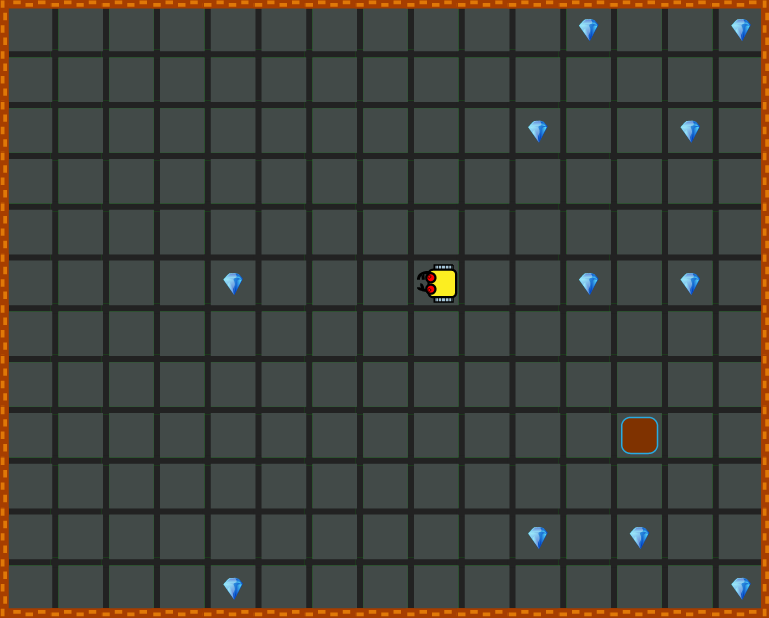
\includegraphics[height=0.4\textwidth]{img/e01.png}
\end{center}
\vspace{-4mm}
\caption{Karel plays hide-and-seek with his friends.}
\label{fig:e02}
\end{figure}
\vspace{-10mm}
\newpage

\subsection{Wall}

{\em Karel stands next to a straight wall of random length and faces a random direction. The wall is not touching the border of the maze. The robot's home square is adjacent to the wall but on the other side. Write a program for the robot to get there!}\\[-7mm]

\begin{figure}[!ht]
\begin{center}
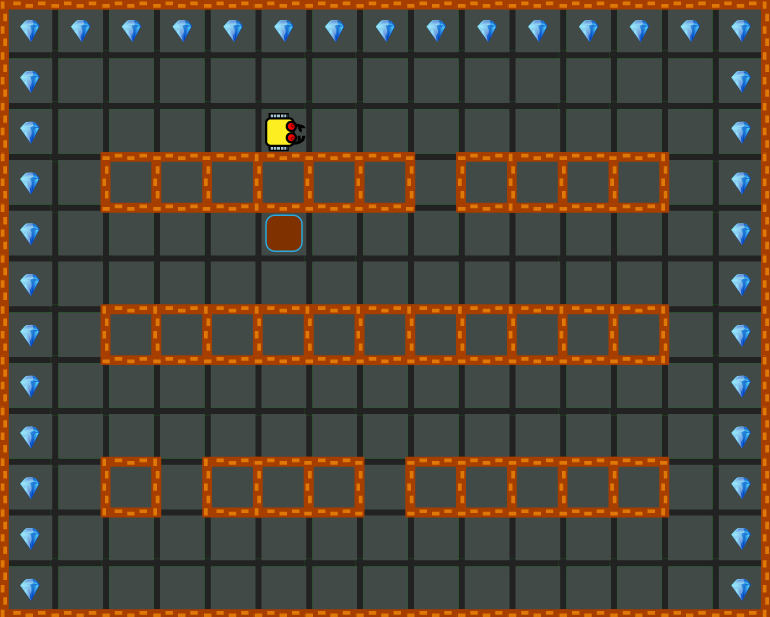
\includegraphics[height=0.4\textwidth]{img/e02.png}
\end{center}
\vspace{-4mm}
\caption{Karel's home square is on the other side of the wall.}
\label{fig:e03}
\vspace{-10mm}
\end{figure}

\subsection{Spiral maze}

{\em Karel stands at the beginning of a spiral maze, facing South. The spiral can be either clock-wise or counter clock-wise oriented. Write a program for Karel to get to his home square, collecting all gems on the way!}\\[-7mm]

\begin{figure}[!ht]
\begin{center}
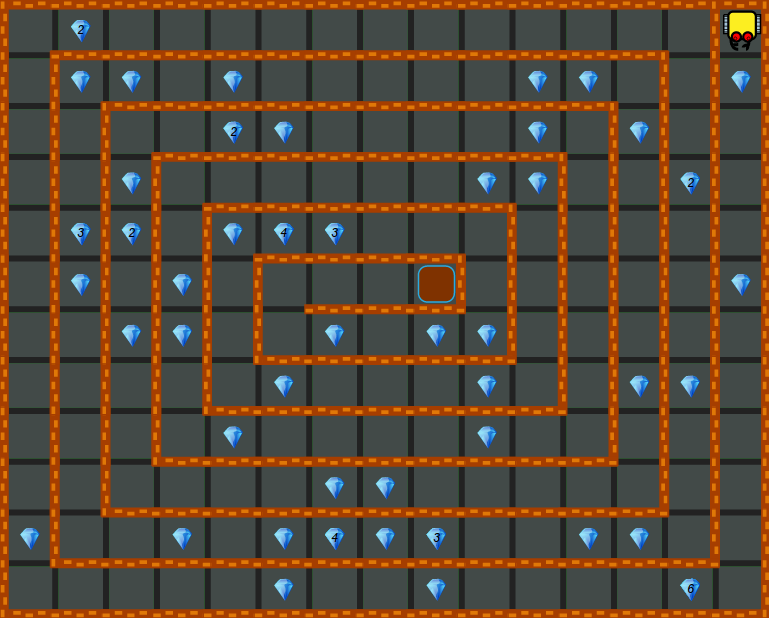
\includegraphics[height=0.4\textwidth]{img/e03.png}
\end{center}
\vspace{-4mm}
\caption{Karel is collecting gems in a spiral maze.}
\label{fig:e04}
\vspace{-10mm}
\end{figure}
\newpage

\subsection{Skyline}

{\em Karel stands in the south-west corner of the maze, facing east. In front of him is an array of poles of random heights. Between some of them, gems lie on the ground. Write a program for the robot to collect all gems and enter his home square!}\\[-7mm]

\begin{figure}[!ht]
\begin{center}
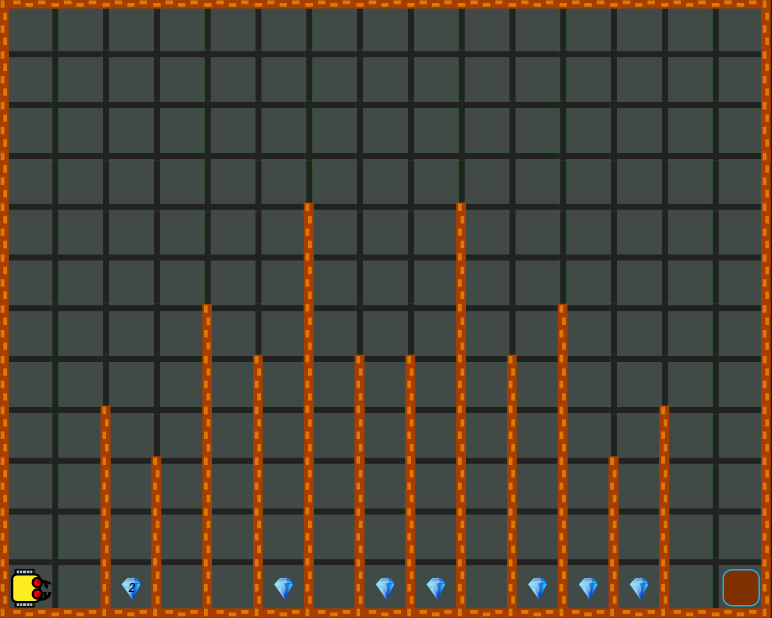
\includegraphics[height=0.4\textwidth]{img/e04.png}
\end{center}
\vspace{-4mm}
\caption{Karel faces an array of randomly-high poles.}
\label{fig:e06}
%\vspace{-10mm}
\end{figure}

%%%%%%%%%%%%%%%%%%%%%%%%%%%%%%%%%%%%%%%%%%%%%%%%%%%%%%%%%%%%%%%%%%%%%%%%%%%%%%%%%%%%%%%%%%

\section{Programming Mode 2 - Custom Commands}

\subsection{Gem jam}

{\em In this maze, gems are distributed randomly along the walls. Otherwise the maze is empty. Karel's home is in the south-west corner, and the robot stands on the right of it, facing east. Write a program for Karel to collect all the gems and return home!}
\newpage

\begin{figure}[!ht]
\begin{center}
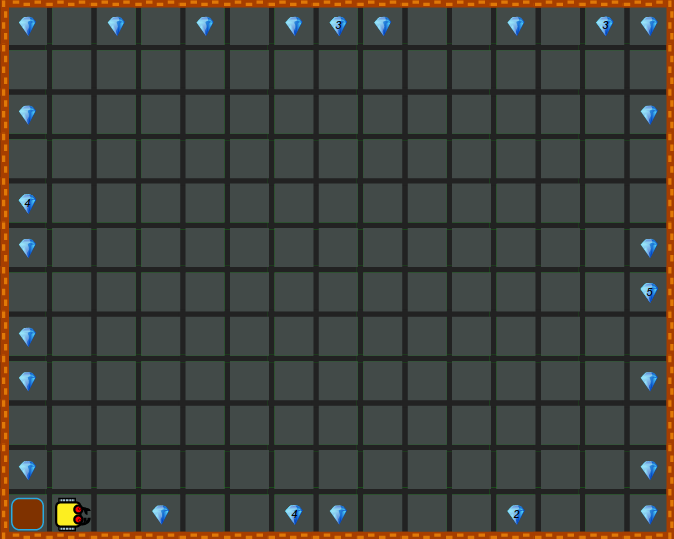
\includegraphics[height=0.4\textwidth]{img/f10.png}
\end{center}
\vspace{-4mm}
\caption{Gems are distributed randomly along the walls.}
\label{fig:f10}
%\vspace{-1cm}
\end{figure}

\subsection{Diamond staircase}

{\em Write a program for Karel to climb the staircase, collect all gems, and enter his home square. The number of steps in the staircase is random.}

\begin{figure}[!ht]
\begin{center}
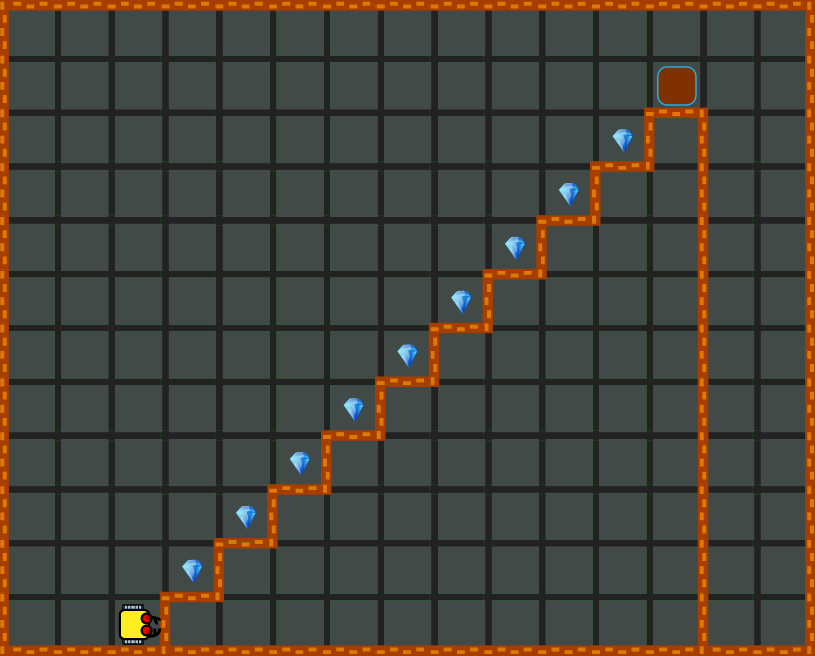
\includegraphics[height=0.4\textwidth]{img/f06.png}
\end{center}
\vspace{-4mm}
\caption{Karel's home is on top of a diamond staircase.}
\vspace{-4mm}
\label{fig:f06}
\end{figure}

\subsection{Pirate ship}

{\em Karel is on a pirate ship! Write a program for the robot to collect all 
gems and run to his home square before the pirates are back. Karel 
needs to be extremely efficient to survive, so there should be 
no repeated code whatsoever in your program!}\\[-9mm]

\begin{figure}[!ht]
\begin{center}
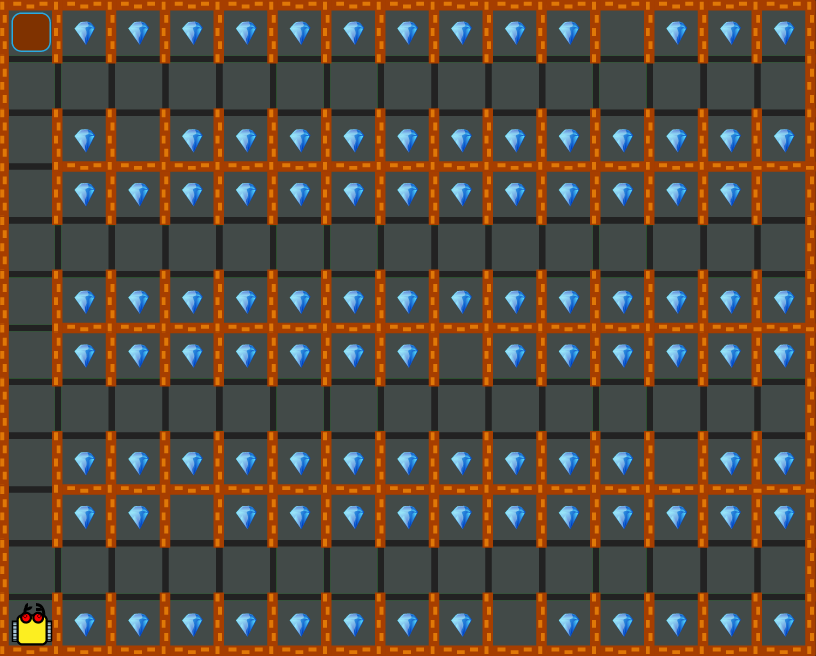
\includegraphics[height=0.4\textwidth]{img/f05.png}
\end{center}
\vspace{-4mm}
\caption{Karel found a pirates' treasure.}
\label{fig:f05}
\vspace{-1.2cm}
\end{figure}

\subsection{Four stars}

{\em Define a custom command to collect one star of gems, and use it four times!}\\[-8mm]

\begin{figure}[!ht]
\begin{center}
\includegraphics[height=0.4\textwidth]{img/f01.png}
\end{center}
\vspace{-4mm}
\caption{Karel needs to collect four stars of gems.}
\label{fig:f01}
\vspace{-10mm}
\end{figure}
\newpage

\subsection{Gems for friends}

{\em Karel needs to return some gems to his friends who live close by. Write a program for the robot to put a gem on the ground in the middle of each friend's home, and then get back to his own house! Define a command to get to the next house and leave a gem there. Repeat it four times.}\\[-7mm]


\begin{figure}[!ht]
\begin{center}
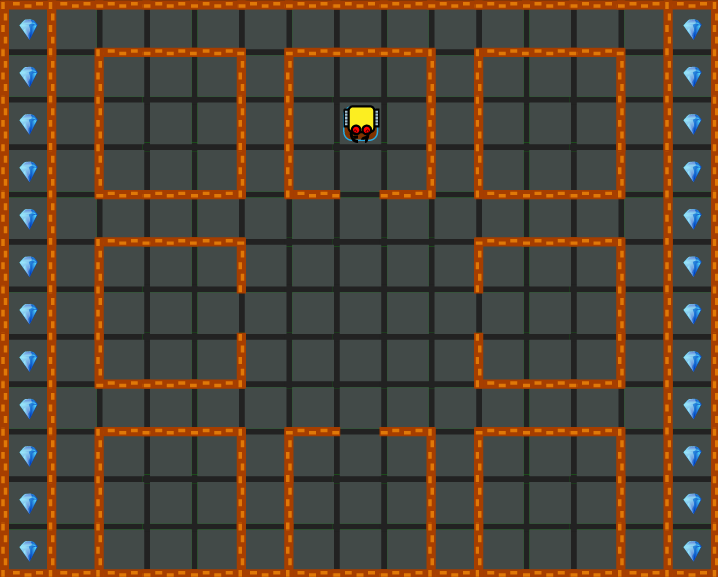
\includegraphics[height=0.4\textwidth]{img/f08.png}
\end{center}
\vspace{-4mm}
\caption{Karel needs to return three gems to his friends.}
\label{fig:f08}
\vspace{-12mm}
\end{figure}

\subsection{Transport}

{\em Write a program for the robot to move a 6x6 square of gems from the north-west
corner to the south-east corner of the maze, and return to his home square.}\\[-7mm]

\begin{figure}[!ht]
\begin{center}
\includegraphics[height=0.4\textwidth]{img/f02.png}
\end{center}
\vspace{-4mm}
\caption{These gems need to be transported to the opposite corner of the maze.}
\label{fig:f02}
\end{figure}
\vspace{-12mm}
\newpage

\subsection{Egg hunt}

{\em There are six cells and each contains several randomly distributed eggs (gems). 
Write a program for Karel to collect all of them!}\\[-9mm]


\begin{figure}[!ht]
\begin{center}
\includegraphics[height=0.4\textwidth]{img/f03.png}
\end{center}
\vspace{-4mm}
\caption{Easter is here, and Karel is on egg hunt.}
\vspace{-1.2cm}
\label{fig:f03}
\end{figure}


\subsection{Pool repair}

{\em Karel stands below the south-west corner of a rectangular pool, facing east. His home square is right behind him. The pool has random dimensions, and it contains a random number of leaks. Each of them is exactly one tile large. Write a program for the robot to seal all leaks by gems and return to his home square!}\\[-9mm]

\begin{figure}[!ht]
\begin{center}
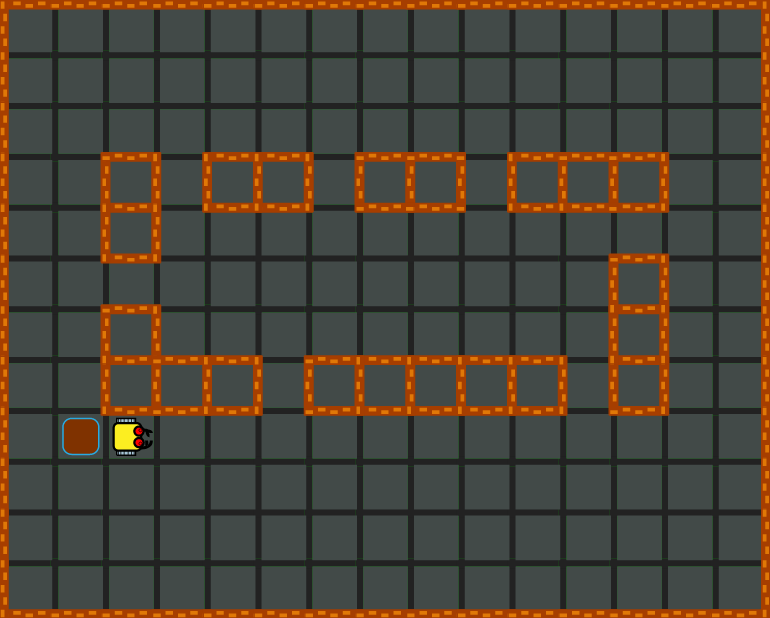
\includegraphics[height=0.4\textwidth]{img/f04.png}
\end{center}
\vspace{-4mm}
\caption{Karel is repairing a leaking pool.}
\label{fig:f04}
\vspace{-1.4cm}
\end{figure}
\newpage

\subsection{Matrix}

{\em Write a program for Karel to collect all gems and enter his home square! Break the task into smaller ones, and define custom commands for these.}\\[-7mm]

\begin{figure}[!ht]
\begin{center}
\includegraphics[height=0.4\textwidth]{img/f11.png}
\end{center}
\vspace{-4mm}
\caption{The Matrix.}
\label{fig:f11}
\end{figure}
\vspace{-1cm}

\subsection{Alcatraz}

{\em Karel is escaping from the Alcatraz prison! At the moment he is in an underground labyrinth with many tunnels but only one of them leads to his freedom. Start by going straight ahead to the nearest wall. Then use the right-hand rule to search the tunnels.}\\[-7mm]

\begin{figure}[!ht]
\begin{center}
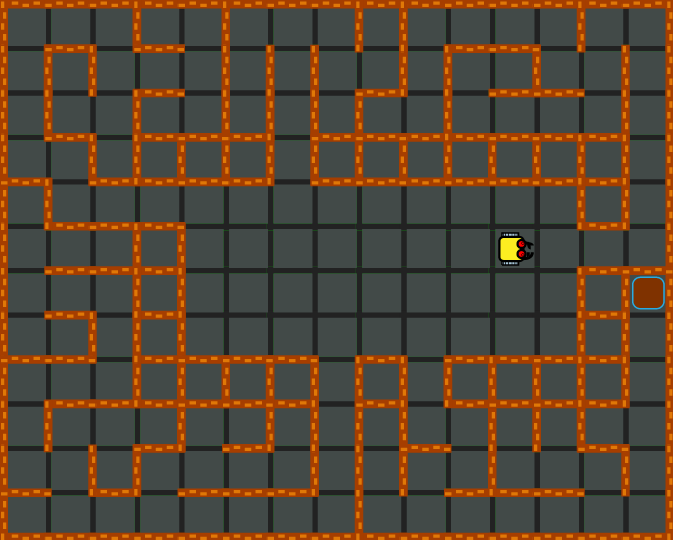
\includegraphics[height=0.4\textwidth]{img/f12.png}
\end{center}
\vspace{-4mm}
\caption{Karel is escaping from the Alcatraz prison.}
\label{fig:f12}
\vspace{-1cm}
\end{figure}
\newpage


\subsection{Border patrol}

{\em Write a program for Karel to check the perimeter of the maze using the 
right-hand rule. Do not forget to pick up all gems that you find on the way.}

\begin{figure}[!ht]
\begin{center}
\includegraphics[height=0.4\textwidth]{img/f13.png}
\end{center}
\vspace{-4mm}
\caption{Border Patrol.}
\label{fig:f13}
\vspace{-1cm}
\end{figure}

\newpage


\subsection{Ariadne I}

{\em In an ancient Greek legend, princess Ariadne saved the life of her beloved Theseus by giving him a thread that he used to avoid getting lost in the maze of king Minos and kill a feared beast Minotaurus. Your task is to write a program for Karel to follow a trail of gems that leads to his home square. The gems form a simple path without loops. There is one additional simplification: Whenever the trail takes a turn, there will be a wall in front of the robot. Do not forget to collect all gems!}


\begin{figure}[!ht]
\begin{center}
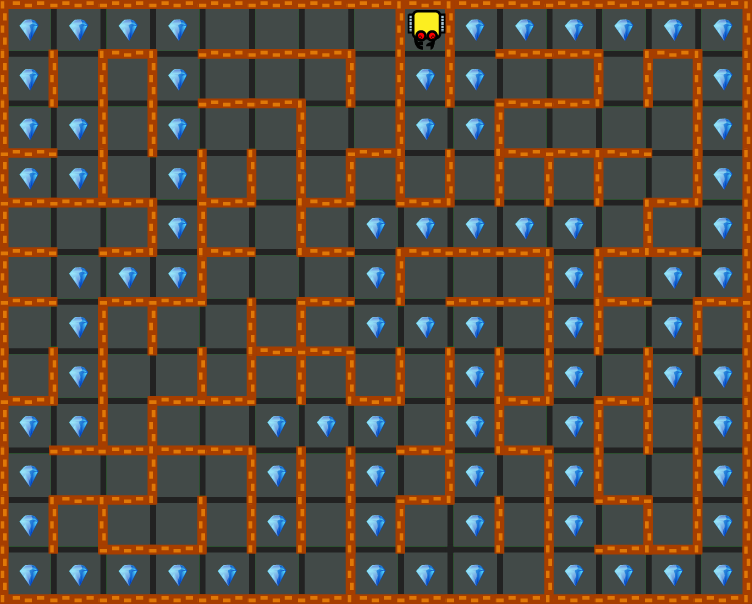
\includegraphics[height=0.4\textwidth]{img/f14.png}
\end{center}
\vspace{-4mm}
\caption{Maze of king Minos, home of the beast Minotaurus.}
\label{fig:f14}
\end{figure}


%%%%%%%%%%%%%%%%%%%%%%%%%%%%%%%%%%%%%%%%%%%%%%%%%%%%%%%%%%%%%%%%%%%%%%%%%%%%%%%%%%%%%%%%%%
\newpage

\section{Programming Mode 3 - Variables and Functions}

\subsection{Accounting}

{\em Karel has an unknown number of gems in his bag. Write a function {\tt accounting} for the 
robot to count the gems and return their number. Then call the function and print the result.}


\begin{figure}[!ht]
\begin{center}
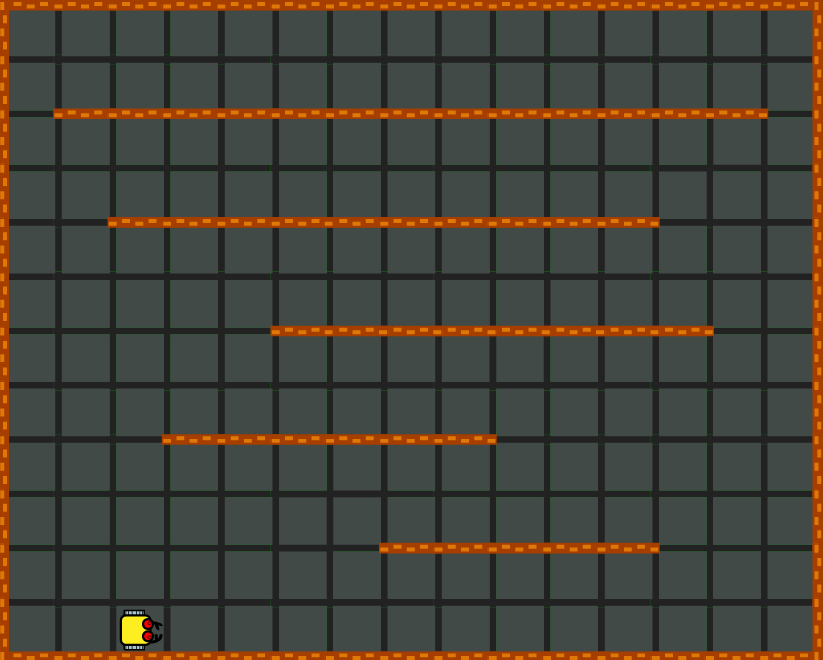
\includegraphics[height=0.4\textwidth]{img/h01.png}
\end{center}
\vspace{-4mm}
\caption{Karel is counting his gems.}
\label{fig:h01}
\end{figure}


\newpage

\subsection{Ariadne II}

{\em This is a continuation of the problem Ariadne I. Your task is to write a program for Karel to follow a trail of gems that leads to his home square. The gems form a simple path without loops. In contrast to Ariadne I, when the trail takes a turn, there may not be a wall in front of the robot. Do not forget to collect all gems!}


\begin{figure}[!ht]
\begin{center}
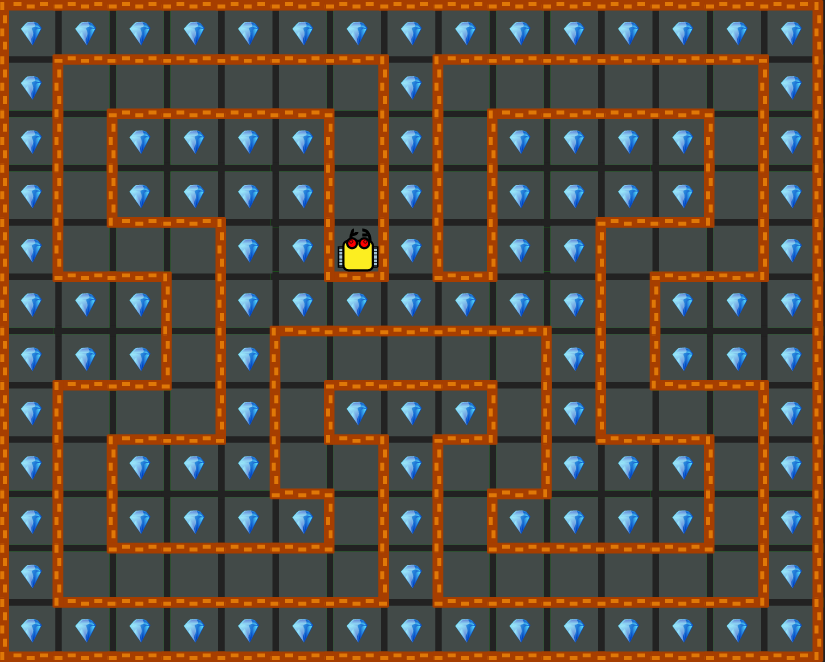
\includegraphics[height=0.4\textwidth]{img/f14k.png}
\end{center}
\vspace{-4mm}
\caption{Now there may not be wall in front of the robot when the trail takes a turn.}
\label{fig:f14k}
\end{figure}
\newpage

%%%%%%%%%%%%%%%%%%%%%%%%%%%%%%%%%%%%%%%%%%%%%%%%%%%%%%%%%%%%%%%%%%%%%%%%%%%%%%%%%%%%%%%%%%

\section{Programming Mode 3 - Lists}

\subsection{Tape measure}

{\em Karel stands in a rectangular room with random dimensions. Write function {\tt measure}  
that returns a list [x, y] where 'x' and 'y' are the horizontal and vertical sizes of the room,
respectively. Call the function and print the result.}

\begin{figure}[!ht]
\begin{center}
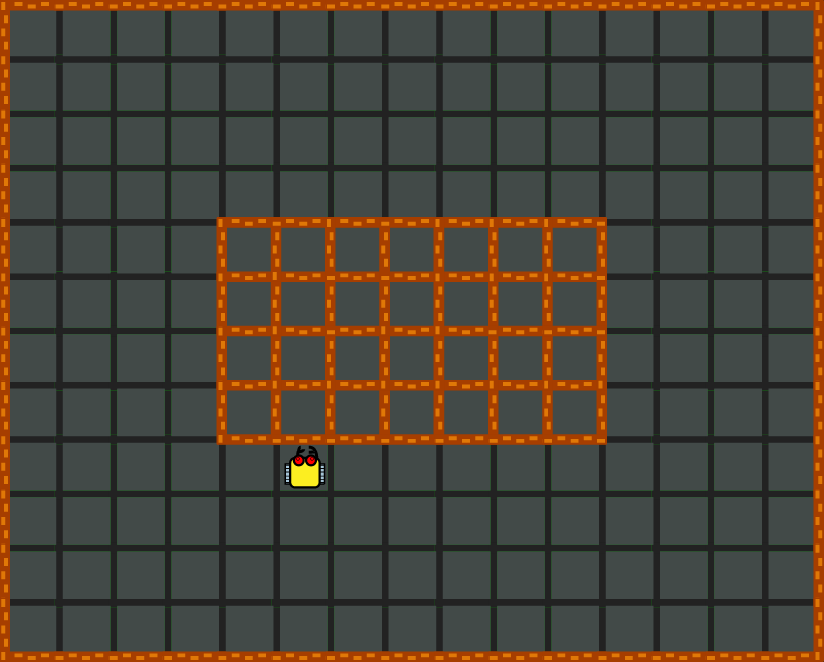
\includegraphics[height=0.4\textwidth]{img/h02.png}
\end{center}
\vspace{-4mm}
\caption{Karel is measuring his room.}
\label{fig:h02}
%\vspace{-1cm}
\end{figure}
%\newpage

\newpage

\subsection{Reconnaissance}

{\em Karel stands in a rectangular room with random dimensions, that contains gems at random positions. There is at most one gem in each square. Write function {\tt gems}  that returns a list of pairs [x, y] where 'x' and 'y' are the GPS coordinates of each gem. Call the function and print the result.}


\begin{figure}[!ht]
\begin{center}
\includegraphics[height=0.4\textwidth]{img/h02b.png}
\end{center}
\vspace{-4mm}
\caption{Karel is locating gems.}
\label{fig:h02b}
\end{figure}


\newpage

\subsection{Orchard}

{\em Trees in Karel's orchard are represented by piles of gems. The position of trees as well as the number of apples per tree are random. Initial position of the robot is in the south-west corner, facing east. There are no walls to crash into. Write a procedure {\tt orchard} for the robot to return a list of triplets [x, y, n] with one triplet per tree, where 'x' and 'y' are the GPS coordinates and 'n' the number of apples on the tree.}


\begin{figure}[!ht]
\begin{center}
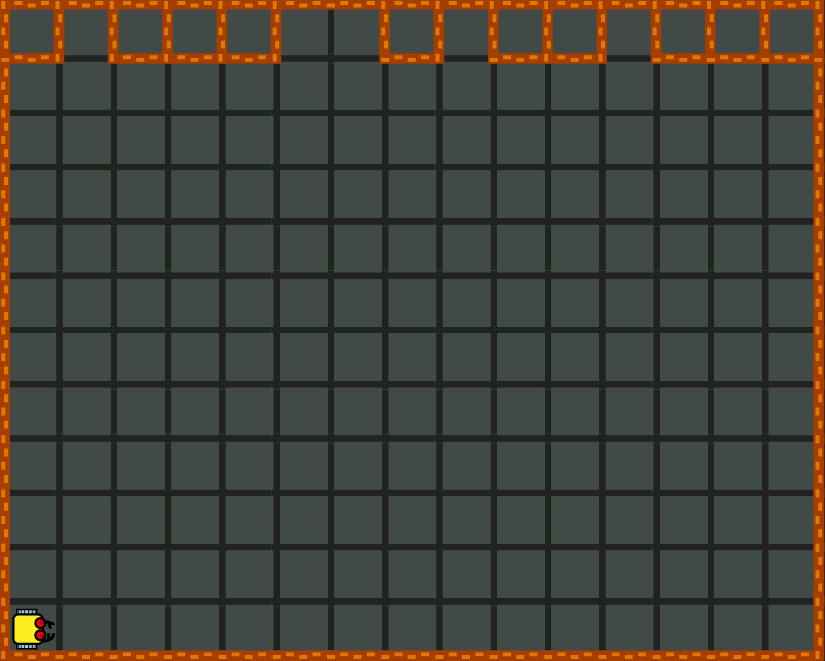
\includegraphics[height=0.4\textwidth]{img/h03.png}
\end{center}
\vspace{-4mm}
\caption{Karel is locating trees and counting apples in his orchard.}
\label{fig:h03}
\end{figure}

\newpage

\subsection{New carpet}

{\em Karel needs new carpet! His apartment has random but simple shape -- wherever 
the robot stands, when he goes north, south, east or west he will always reach exterior wall.
The initial position of the robot is at the west wall of the bottom row, facing east. 
Write a function {\tt carpet} that returns a list of triplets [x, y, n] with one triplet for each
row, starting with the bottom one, where 'x' and 'y' are the GPS coordinates of the left-most
square, and 'n' is the size of the row. }

\begin{figure}[!ht]
\begin{center}
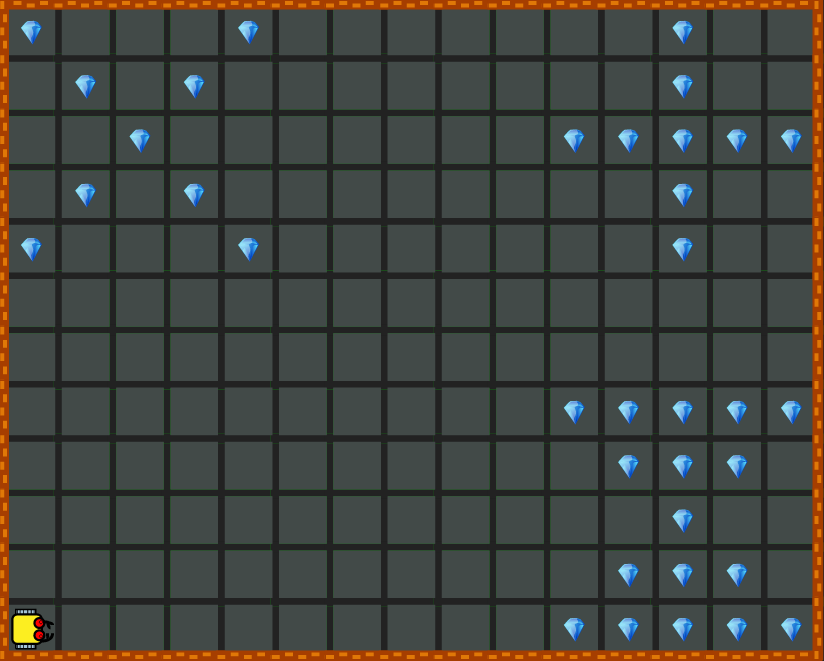
\includegraphics[height=0.4\textwidth]{img/h04.png}
\end{center}
\vspace{-4mm}
\caption{Karel is measuring his apartment before buying new carpet.}
\vspace{-1cm}
\label{fig:h04}
\end{figure}




%%%%%%%%%%%%%%%%%%%%%%%%%%%%%%%%%%%%%%%%%%%%%%%%%%%%%%%%%%%%%%%%%%%%%%%%%%%%%%%%%%%%%%%%%%
\newpage
\section{Programming Mode 3 - Logic and Randomness}

\subsection{Reading numbers}

{\em Each 3x5 box contains a random integer number between 0 and 9. Write a function "readnumber" 
where Karel enters a box, determines the number in it, and returns it. Initial position of the 
robot is at the entrance of the box, facing north. The final position of the robot should be the same. 
Use this function to determine the numbers in the three boxes as shown in the screenshot. }

\begin{figure}[!ht]
\begin{center}
\includegraphics[height=0.4\textwidth]{img/i01.png}
\end{center}
\vspace{-4mm}
\caption{Karel is learning to read numbers.}
\label{fig:g10}
\end{figure}


\newpage

\subsection{Writing numbers}

{\em There is a pile of gems at the entrance of each box. The number of gems in each pile is random between 0 and 9. Write a function "writenumber" where Karel counts the gems in the pile, enters the box, and renders the number. Then use the function to render numbers in three boxes as shown in the screenshot. }


\begin{figure}[!ht]
\begin{center}
\includegraphics[height=0.4\textwidth]{img/i02.png}
\end{center}
\vspace{-4mm}
\caption{Karel is learning to write numbers.}
\label{fig:g11}
\vspace{-10mm}
\end{figure}


\newpage

\subsection{Adding numbers}

\noindent
{\em This problem can be solved with the help of the results 
of the previous two exercises.
The two upper boxes contain randomly generated numbers between 0 and 9. Karel stands at the entrance of the first box,
facing north. Write a function {\tt addnumbers} where Karel will enter each box, determine the number in it,
and then add the numbers together and return the result. Also render the result in the double-box below. 
Use the functionality developed in the previous two tasks!}

\begin{figure}[!ht]
\begin{center}
\includegraphics[height=0.4\textwidth]{img/i03.png}
\end{center}
\vspace{-4mm}
\caption{Karel is adding randomly generated numbers.}
\label{fig:g12}
\end{figure}

%%%%%%%%%%%%%%%%%%%%%%%%%%%%%%%%%%%%%%%%%%%%%%%%%%%%%%%%%%%%%%%%%%%%%%%%%%%%%%%%%%%%%%%%%%
\newpage

\section{Programming Mode 3 - Recursion}

\subsection{Cheese please}

{\em Karel's favorite way to eat cheese is to peel one edge at a time. His brick of 
cheese is represented by a rectangle of gems. The rectangle has random dimensions
and the robot's initial position is at one of the corners, as shown in Fig. \ref{fig:g01}.
Write a recursive algorithm for the robot to eat all the cheese and return home!
 }
\begin{figure}[!ht]
\begin{center}
\includegraphics[height=0.4\textwidth]{img/g01.png}
\end{center}
\vspace{-4mm}
\caption{Karel is eating cheese.}
\label{fig:g01}
\vspace{-1cm}
\end{figure}
\newpage


\subsection{Speleologist}

{\em Karel stands at the entrance to a cave and wants to explore it. Write a recursive program for the robot to descend the staircase to the bottom, return back, and enter his home! The number of steps in the staircase is random.}
\begin{figure}[!ht]
\begin{center}
\includegraphics[height=0.4\textwidth]{img/g02.png}
\end{center}
\vspace{-4mm}
\caption{Karel became a speleologist.}
\label{fig:g02}
\end{figure}
\vspace{-1cm}



\subsection{Homage to lemmings}

{\em  Karel has many gems in his bag, and he needs to build a heap shown in Fig. \ref{fig:g03} before he can 
enter his home. Use recursion.}

\begin{figure}[!ht]
\begin{center}
\includegraphics[height=0.4\textwidth]{img/g03.png}
\end{center}
\vspace{-4mm}
\caption{Karel needs to build a heap of gems before he can get home.}
\label{fig:g03}
\vspace{-1cm}
\end{figure}
\newpage


\subsection{Diamond tree}

{\em Karel stands under a diamond tree, with his home next to him on the the right. 
The tree is random -- at any point it can have 
a branch in the north-west or in the north-east direction (or in both). Write a recursive 
algorithm for the robot to collect all gems from the tree and get home!  }

\begin{figure}[!ht]
\begin{center}
\includegraphics[height=0.4\textwidth]{img/g04.png}
\end{center}
\vspace{-4mm}
\caption{Karel is traversing a random diamond tree.}
\label{fig:g04}
\vspace{-10mm}
\end{figure}


\newpage

\section{Programming Mode 3 - Advanced Programs}

If the previous exercises have not been challenging enough, then here is something 
for you. Enjoy!

\subsection{Eight queens}

\noindent
{\em Karel stands on an 8 x 8 chess board along with eight queens (gems). Recall that a chess queen dominates its row, its column, as well as both diagonals that pass through her position. Nothing may stand in these fields or she will destroy it. Currently, some queens are threatening each other. Write a program for Karel to correct the positions of the queens in such a way that none of them is threatened. You can assume that each column and each row contains exactly one queen. }

\begin{figure}[!ht]
\begin{center}
\includegraphics[height=0.4\textwidth]{img/i04.png}
\end{center}
\vspace{-4mm}
\caption{The eight queens problem.}
\label{fig:g14}
\end{figure}

\newpage
\subsection{Bubble sort}

\noindent
{\em Karel stands in front of 9 piles of gems. Each pile contains a random number of gems between 1 and 9. 
Two or more piles can be equally large. Sort the piles in such a way that the smallest pile is on the left 
and the largest on the right. Hint -- look up the BubbleSort algorithm on Wikipedia.}

\begin{figure}[!ht]
\begin{center}
\includegraphics[height=0.4\textwidth]{img/i05.png}
\end{center}
\vspace{-4mm}
\caption{BubbleSort algorithm.}
\label{fig:g13}
\end{figure}

\newpage
\subsection{Land surveyor}

\noindent
{\em Karel took a job as land surveyor and his first task is to measure the size of a fenced property. However, there is a big dog inside and Karel is scared of dogs. If he fails to measure the size of the property, he will lose his job. Hence, you need to write a program for the robot to calculate the size of the property without actually entering it. You can assume that the fence does not touch the boundary of the maze and that Karel is free to walk along the entire length of the fence. The property has a random shape and the robot is standing next to the fence.}

\begin{figure}[!ht]
\begin{center}
\includegraphics[height=0.4\textwidth]{img/j01.png}
\end{center}
\vspace{-4mm}
\caption{Karel needs to measure the size of the property without entering it.}
\label{fig:j01}
\end{figure}

\newpage
\subsection{Loopy loop}

\noindent
{\em Write a program for Karel to decide whether the walls in the maze form a closed loop or not. You can assume that the robot can freely walk along all walls and that they do not touch the maze's boundary.  }

\begin{figure}[!ht]
\begin{center}
\includegraphics[height=0.4\textwidth]{img/j03.png}
\end{center}
\vspace{-4mm}
\caption{Karel needs to decide whether the curve is open or closed.}
\label{fig:j03}
\end{figure}


\newpage
\subsection{Espionage}

\noindent
{\em Karel works for the Secret Service. The word is out that 
enemy spies may be hiding in the maze. The rumor has it that they are 
hiding in a place that is completely surrounded with walls and thus 
not reachable from any direction. Hence, your task is to write a program 
for the robot to traverse the entire maze and decide whether all positions 
are reachable or not. Return a list containing all unreachable positions 
(the list should be empty if there are none). This list will be used by 
an assault team to eliminate all enemy forces.}

\begin{figure}[!ht]
\begin{center}
\includegraphics[height=0.4\textwidth]{img/j02.png}
\end{center}
\vspace{-4mm}
\caption{Karel is looking for hidden spies.}
\label{fig:j02}
\end{figure}
\noindent

